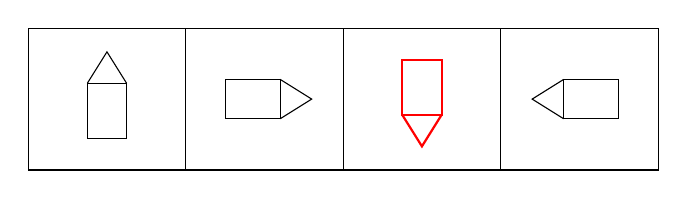
\begin{tikzpicture}[x=1cm,y=1cm]\draw (0,0) rectangle(8,1.8);\foreach \x in {2,4,6}{\draw(\x,0)--(\x,1.8);}\foreach \x/\a in {1/0,3/-90,7/90}{\begin{scope}[shift={(\x,.9)},rotate=\a]\draw(-.25,-.5) rectangle(.25,.2);\draw(-.25,.2)--(0,.6)--(.25,.2);\end{scope}}
\begin{scope}[shift={(5,.9)},rotate=180]\draw[red,thick](-.25,-.5)rectangle(.25,.2);\draw[red,thick](-.25,.2)--(0,.6)--(.25,.2);\end{scope}
\end{tikzpicture}
